\documentclass[10pt,a4paper]{article}
\usepackage[utf8]{inputenc}
\usepackage[spanish]{babel}
\usepackage{amsmath}
\usepackage{amsfonts}
\usepackage{amssymb}
\usepackage{graphics}
\usepackage{graphicx}
\usepackage{xcolor}
\usepackage{listings}
\usepackage{csvsimple}
\usepackage{caption}
\usepackage{subcaption}
\usepackage[left=2cm,right=2cm,top=2cm,bottom=2cm]{geometry}

\renewcommand*\contentsname{Índice} %Nombre del indice

\begin{document}
\lstset{
	basicstyle=\footnotesize,
	extendedchars=true,
	literate={á}{{\'a}}1 {ã}{{\~a}}1 {é}{{\'e}}1 {ú}{{\'u}}1 {ó}{{\'o}}1,
	backgroundcolor=\color{black!5}
	}
	
\begin{titlepage}
	\centering
	{
\includegraphics[scale=0.5]{Logo_UGR.png}\par}
	\vspace{1cm}
	{\bfseries\Large Escuela T\'ecnica Superior de Ingeniería Informática y Telecomunicaciones \par}
	\vspace{2.5cm}
	{\scshape\Huge Pr\'actica 2: Divide y Vencerás \par}
	\vspace{3cm}
	{\itshape\Large Doble Grado Ingeniería Informática y Matemáticas}
	\vfill
	{\Large Autores: \par}
	{\Large Jose Alberto Hoces Castro\par}
	{\Large Javier Gómez López \par}
	{\Large Moya Mart\'in Castaño \par}
	\vfill
	{\Large Abril 2022 \par}
\end{titlepage}

\thispagestyle{empty}
\null
\vfill

%%Información sobre la licencia
\parbox[t]{\textwidth}{
  
\includegraphics[scale=0.05]{by-nc-sa.png}\\[4pt]
  \raggedright % Texto alineado a la izquierda
  \sffamily\large
  {\Large Este trabajo se distribuye bajo una licencia CC BY-NC-SA 4.0.}\\[4pt]
  Eres libre de distribuir y adaptar el material siempre que reconozcas a los\\
  autores originales del documento, no lo utilices para fines comerciales\\
  y lo distribuyas bajo la misma licencia.\\[4pt]
  \texttt{creativecommons.org/licenses/by-nc-sa/4.0/}
}

\newpage

\tableofcontents

\newpage
\section{Introducción}

El objetivo de esta práctica es utilizar la técnica ``divide y vencerás'' para resolver problemas de forma más eficiente que otras alternativas más sencillas o directas. Para ello, se plantean los siguientes dos problemas:

\begin{itemize}
	\item \textbf{Ejercicio 1:} Este problema consiste en realizar la búsqueda de un elemento en un vector ordenado con \(n\) elementos.
	\item \textbf{Ejercicio 2:} Este problema consiste en dados \(k\) vectores de \(n\) elementos, todos ellos ordenados de menor a mayor, combinar todos los vectores en uno único ordenado.
\end{itemize}

\section{Desarrollo}

Para los análsis de algoritmos que nos pedirán más adelante, hemos realizado los siguientes pasos:
\begin{enumerate}
	\item Un \textbf{análisis teórico} de los algoritmos usando las técnicas vistas en clase.
	\item Un \textbf{análisis empírico} donde hemos ejecutado los algoritmos en nuestros ordenadores bajo las misma normas y condiciones. Hemos compilado usando la compilación  \texttt{-Og}. Además hemos usado como \textit{datasets} de pruebas generadores de datos aleatorios proporcionados por la profesora. Por otro lado, para automatizar el proceso, hemos generado unos \textit{scripts} de generación de datos de prueba y de ejecución de nuestros programas. Hemos ejecutado cada algoritmo 15 veces en cada uno de los tamaños que han sido probados, y hemos hecho la media de ellos para reducir perturbaciones que puedan alterar el resultado.
	\item Un \textbf{análisis híbrido} donde hemos tomado los datos de cada uno de los alumnos del grupo y hemos hallado la \(K\) (constante oculta). Para ello hemos usado gnuplot.
\end{enumerate}

\subsection{Ejercicio 1}
El enunciado del problema es el siguiente: \textit{Dado un vector ordenado (de forma no decreciente) de números enteros \(v\), todos distintos, el objetivo es determinar si existe un índice \(i\) tal que \(v[i] = i\) y encontrarlo en ese caso. Diseñar e implementar un algoritmo ``divide y vencerás'' que permita resolver el problema. ¿Cuál es la complejidad de ese algoritmo y la del algoritmo ``obvio'' para realizar esta tarea? Realizar también un estudio empírico e híbrido de la eficiencia de ambos algoritmos.}

\textit{Supóngase ahora que los enteros no tienen por qué ser todos distintos (pueden repetirse). Determinar si el algoritmo anterior sigue siendo válido, y en caso negativo proponer uno que sí lo sea. ¿Sigue siendo preferible al algoritmo obvio?}

\subsubsection{Algoritmo de fuerza bruta}
La manera obvia de resolver este ejercicio sería mediante un algoritmo secuencial, que vaya recorriendo el vector hasta encontrar el elemento buscado. Pasemos a realizar un análisis de este algoritmo:

\begin{enumerate}
	\item \textbf{Análisis Teórico}
	
	\lstinputlisting[language=C++]{./Codes/secuencial.cpp}
	
	Tal y como se ha indicado en los comentarios del código, todas las operaciones de asignación y comprobación de los \texttt{if} son \(\mathcal{O}(1)\). Estas, a sus vez, se incluyen dentro de un bucle \texttt{for}. Dicho bucle es \(\mathcal{O}(n)\), obteniendo así que la función \texttt{int buscarSecuencial} es \(\mathcal{O}(n)\), es decir
	\[
	T(n) \in \mathcal{O}(n)
	\]
	
	\item \textbf{Análisis Empírico}
	
	Tras ejecutar el algoritmo para 26 tamaños distintos; desde 1000000 hasta 20000000 dando saltos de 760000, hemos obtenido los siguientes resultados:
	
	\begin{table}[h!]
	\centering
	\footnotesize
	\scalebox{0.75}{
		\begin{tabular}{|c|c|}
			\hline
			\multicolumn{2}{|c|}{\textsf{Algoritmo de fuerza bruta}}
			\\\hline
			\bfseries Elementos (n) & \bfseries Tiempo (s)
			\csvreader{./data/secuencial.csv}{}
			{\\\hline\csvcoli&\csvcolii}
			\\\hline
		\end{tabular}
	}
	\caption{Experiencia empírica de la búsqueda a fuerza bruta}
    \end{table}

	\item \textbf{Análisis Híbrido}
	
	A continuación, aprovechamos los tiempos obtenidos en el análisis empírico para hallar la función de ajuste, para lo cual hemos hecho uso de gnuplot de la misma forma que en la anterior práctica. He aquí la gráfica correspondiente:
	
	\begin{figure}[h!]
		\centering
		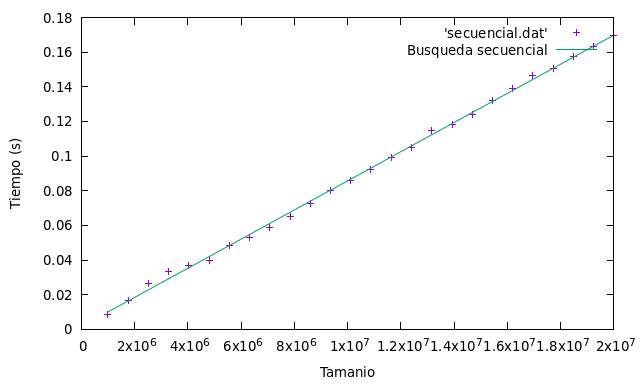
\includegraphics[scale=0.55]{./Images/Grafica_secuencial.png}
		\caption{Gráfica con los tiempos de ejecución de la búsqueda a fuerza bruta}
	\end{figure}

	Y las constantes ocultas obtenidas son:
	
	\( T(n) = 8.41755 \cdot 10^{-9} n + 0.00153755\).
	
	Y el coeficiente de determinación es:
	
	Coef.determinación = 0.9992
	
	Verificando así que nuestro análisis teórico es correcto.
\end{enumerate}

\subsubsection{Divide y Vencerás}
La oportunidad para usar la técnica ``Divide y Vencerás'' ocurre en el momento en el que trabajamos con vectores ordenados (en nuestro caso de manera creciente). Esto nos permite usar un algoritmo que se basa en la técnica ``Divide y Vencerás'': la búsqueda binaria.

La búsqueda binaria consiste en ir comprobando los elementos del vector comenzado por su mitad. Al estar el vector ordenado, si el valor que hemos comprobado es mayor que la posición en la que se encuentra, podemos desechar la mitad superior de nuestro vector. En caso de ser menor que la posición en la que se encuentra, podemos desechar la primera mitad del vector.  Aplicando esto de manera recursiva, obtenemos un algoritmo de características muy buenas e interesantes. Pasemos a su análisis:

\begin{enumerate}
 \item \textbf{Análisis Teórico}
 
 \lstinputlisting[language=C++]{./Codes/binaria.cpp}
 
 Como podemos observar en los comentarios del código, todas las operaciones son \(\mathcal{O}(1)\) y la llamada recursiva a la función es \(\mathcal{O}\left(\frac{n}{2}\right)\). Una de las dos llamadas recursivas nunca se ejecuta, es decir, vamos descartando mitades del vector, por lo que la recurrencia que expresa el tiempo a partir del tamaño del vector viene dada por la siguiente expresión, de la cual vamos a deducir la eficiencia del algoritmo:
 
 \[
 T(n) = T\left(\frac{n}{2}\right) + a
 \]
 
 Para resolver esta recurrencia, tomamos $n = 2^k$, quedándose de la forma:
 
  \[
 T(2^k) = T(2^{k-1}) + a
 \]
 
 Cuyo polinomio característico es:
 
 \[
 (x-1)^2
 \]
 
 De donde se deduce que la solución de la recurrencia será de la forma $(c0 + c1 \cdot k) \cdot 1^k$, y al deshacer el cambio $n = 2^k$, obtenemos que:
 
 \[
 T(n) = c0 + c1 \cdot \log_{2}(n)
 \]
 
 Por lo que concluimos que:
 
 \[
 	T((n) \in \mathcal{O}(log_{2}(n))
 \]
 
 \item \textbf{Análisis Empírico}\\
 \\
 Tras ejecutar el algoritmo para 26 tamaños distintos; desde 1000000 hasta 20000000 dando saltos de 760000, hemos obtenido los siguientes resultados:
 
 \newpage
 
 \begin{table}[h!]
 	\centering
 	\footnotesize
 	\scalebox{0.75}{
 		\begin{tabular}{|c|c|}
 			\hline
 			\multicolumn{2}{|c|}{\textsf{Divide y Vencerás sin repeticiones}}
 			\\\hline
 			\bfseries Elementos (n) & \bfseries Tiempo (s)
 			\csvreader{./data/binaria.csv}{}
 			{\\\hline\csvcoli&\csvcolii}
 			\\\hline
 		\end{tabular}
 	}
 	\caption{Experiencia empírica de la búsqueda binaria}
 \end{table}
 
 \item \textbf{Análisis híbrido}\\
 \\
 El análisis híbrido nos permitirá comprobar que nuestro análisis teórico era correcto. Usando los datasets del anterior apartado, hemos usado gnuplot para graficar los puntos obtenidos junto con su función de ajuste. A continuación mostramos la gráfica con su respectiva función de ajuste:
 
 \begin{figure}[h!]
 	\centering
 	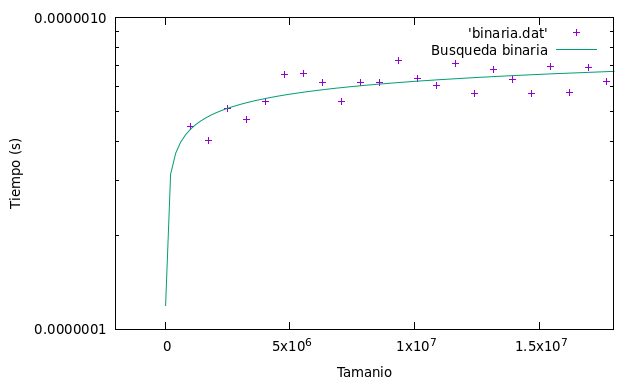
\includegraphics[scale=0.55]{./Images/Grafica_binaria.png}
 	\caption{Gráfica con los tiempos de ejecución de la búsqueda binaria}
 \end{figure}
 
 Y las constantes ocultas son:
 
 \( T(n) = 5.63832 \cdot 10^{-8} \cdot \log_{2}(n) - 6.87177 \cdot 10^{-7}\).
 
 Para terminar nuestro análisis de este algoritmo, terminaremos de confirmar que el ajuste logarítmico es el óptimo viendo el coeficiente de determinación que nos ha proporcionado gnuplot:
 
 Coef.determinación = 0.999999954166
 
 \item \textbf{Comparación algoritmo de fuerza bruta vs Divide y Vencerás sin repeticiones}\\
 
 Como ya sabemos de la práctica anterior, el orden de eficiencia $\mathcal{O}(log_{2}(n))$ es mejor que $\mathcal{O}(n)$, por lo que nuestra implementación usando la técnica ``Divide y Vencerás'' mejora los tiempos de ejecución considerablemente. Para saber a partir de qué tamaño del vector nos renta usar más la búsqueda por fuerza bruta o la nueva implementación, hemos de calcular el \textbf{umbral}, que surge de igualar las expresiones halladas en el análisis híbrido de ambos algoritmos:
 
 \[
 5.63832 \cdot 10^{-8} \cdot \log_{2}(n) - 6.87177 \cdot 10^{-7} = 8.41755 \cdot 10^{-9} n + 0.00153755
 \]
 
 Sin embargo, no existe ningún natural tal que se cumpla esta igualdad, pues la función del algoritmo de fuerza bruta siempre va a estar por encima, luego el umbral es $n = 1$. Por último, mostramos la gráfica comparando las dos funciones de ajuste de ambos algoritmos:
 
 
  \begin{figure}[h!]
 	\centering
 	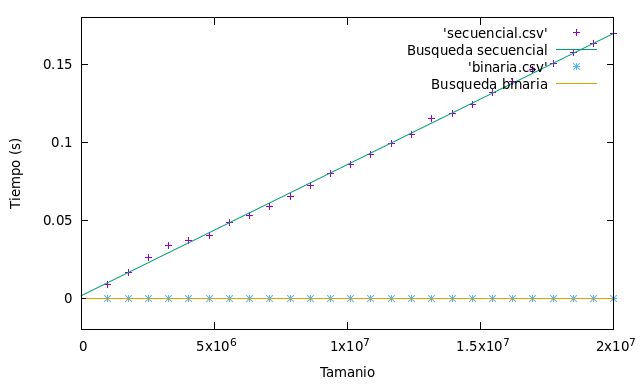
\includegraphics[scale=0.55]{./Images/Grafica_secvsbin.png}
 	\caption{Gráfica comparativa: Fuerza Bruta vs DyV sin repeticiones}
 \end{figure}
\end{enumerate}

\begin{enumerate}
\subsubsection{¿Elementos repetidos?}
Otra parte que se nos plantea en el ejercicio es la siguiente: ¿qué pasaría si en el elemento tuviésemos elementos repetidos? En este caso, la búsqueda binaria tal y como la programamos antes dejaría de ser efectiva. Aquí un ejemplo:
\[
	1 \quad 2 \quad 3 \quad 4 \quad 4 \quad 5 \quad 6 \quad 7
\]

En este caso, el primer elemento que comprobaría nuestro algoritmo sería \(v[3] = 4\). Entonces, desecharía los siguiente elementos a partir de \(v[3]\). Pero vemos que en \(v[4] = 4\), que es el elemento que deseamos. 

Para evitar este problema, hemos diseñado la siguiente solución:

\lstinputlisting[language=C++]{./Codes/binaria_repes.cpp}

\item \textbf{Análisis teórico}\\

Con este algoritmo, obtenemos la siguiente ecuación de recurrencia:
\[
	T(n) = 2 \cdot T \left( \frac{n}{2} \right) + a
\]

Resolviéndola mediante los métodos vistos en clase, tomamos $n = 2^k$ y obtenemos que el polinomio característico asociado a la recurrencia es:

\[
	(x-1)(x-2)
\]

De donde se obtiene que el tiempo se expresa en función de k como:

\[
	T(2^k) = c0 + c1*2^k
\]

Y deshaciendo el cambio obtenemos que $T(n) = c0 + c1*n$, por lo que concluimos que:

\[
	T(n) \in \mathcal{O}(n)
\]

Vemos que es el mismo orden de eficiencia que la búsqueda secuencial. Esto ocurre porque nuestro peor caso es en el que el elemento que buscamos está en \(v[n-2]\). Puesto que vamos comprobando elementos siempre en las mitades inferiores hasta que encontramos lo deseado, para llegar a el elemento \(v[n-2]\) tendríamos que hacer \(n\) iteraciones. Además, este algoritmo es incluso peor que la búsqueda secuencial, ya que en vectores muy grandes podemos llenar la pila de llamadas y hacer nuestro programa imposible de ejecutar. Esto también se ve en los datasets obtenidos en el análisis empírico y en la gráfica comparativa, que veremos a continuación en el análisis empírico e híbrido

\item \textbf{Análisis empírico}\\

Al igual que para el algoritmo de fuerza bruta y el anterior, hemos probado para 26 tamaños distintos (15 repeticiones por tamaño), desde 1000000 hasta 20000000, dando saltos de 760000, dando lugar a este dataset:

\begin{table}[h!]
	\centering
	\footnotesize
	\scalebox{0.75}{
		\begin{tabular}{|c|c|}
			\hline
			\multicolumn{2}{|c|}{\textsf{Divide y Vencerás con repeticiones}}
			\\\hline
			\bfseries Elementos (n) & \bfseries Tiempo (s)
			\csvreader{./data/binaria_repes.csv}{}
			{\\\hline\csvcoli&\csvcolii}
			\\\hline
		\end{tabular}
	}
	\caption{Experiencia empírica de la búsqueda con repeticiones}
\end{table}

\item \textbf{Análisis híbrido}\\

A partir del dataset anterior, hemos usado gnuplot para comprobar que la función de ajuste se corresponde con el orden de eficiencia hallado, corroborando así nuestro análisis. He aquí la gráfica:

 \begin{figure}[h!]
	\centering
	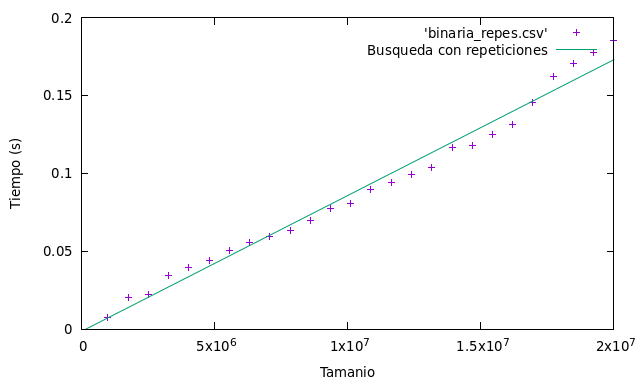
\includegraphics[scale=0.55]{./Images/Grafica_binaria_repes.png}
	\caption{Gráfica con los tiempos de ejecución de la búsqueda con repeticiones}
\end{figure}

Y las constantes ocultas son:

\( T(n) = 8.71886 \cdot 10^{-9} \cdot n -0.00140853 \).

Para terminar nuestro análisis de este algoritmo, terminaremos de confirmar que el ajuste lineal es el óptimo viendo el coeficiente de determinación que nos ha proporcionado gnuplot:

Coef.determinación = 0.9941

\item \textbf{Comparación algoritmo de fuerza bruta vs Divide y Vencerás con repeticiones}\\

Como hemos visto, tanto el algoritmo de fuerza bruta como el ``Divide y Vencerás'' para vectores ordenados con repeticiones presentan una eficiencia $\mathcal{O}(n)$. Además si observamos sus respectivas funciones de ajuste y las graficamos observamos que el algoritmo de fuerza bruta es más eficiente que el ``Divide y Vencerás'' implementado, pues la pendiente del de fuerza bruta es algo menor que la del otro algoritmo:

\begin{figure}[h!]
	\centering
	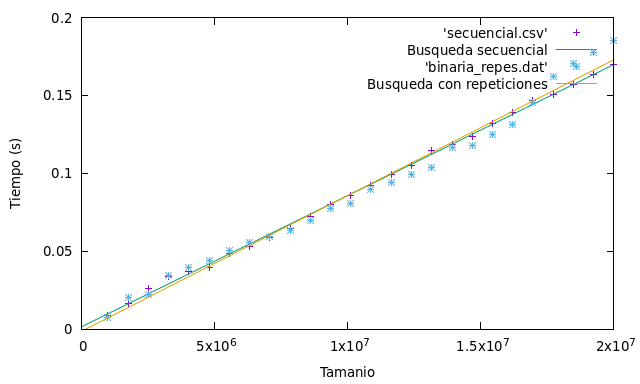
\includegraphics[scale=0.55]{./Images/Grafica_secvsrep.png}
	\caption{Gráfica comparativa: Fuerza Bruta vs DyV con repeticiones}
\end{figure}


Fuerza bruta $\longrightarrow$ \( T(n) = 8.41755 \cdot 10^{-9} n + 0.00153755\).

DyV con repeticiones $\longrightarrow$ \( T(n) = 8.71886 \cdot 10^{-9} \cdot n -0.00140853 \).

El estudio de este caso nos ha servido para obtener una de las conclusiones de nuestro trabajo, y es que la técnica ``Divide y Vencerás'' no siempre da resultado e incluso puede dar lugar a algoritmos que tarden más en dar la solución que lo que tarda el de fuerza bruta.

\end{enumerate}



\subsection{Ejercicio 2}

\subsubsection{Algoritmo de fuerza bruta}

\subsubsection{Divide y Vencerás}
\end{document}